% =====================================================================
%  Sections 4--7: Weak solutions, Non-uniqueness, Entropy condition,
%  Riemann problem.
% =====================================================================

\section{Weak Solutions}
\label{sec:weak-solutions}

From here on we assume $u_0\in L^\infty(\mathbb{R})$, whereas Sections~\ref{sec:characteristics}--\ref{sec:shock-formation}
allowed unbounded $C^1$ data; weak solutions are bounded by
Definition~\ref{def:weak-solution}, so they do not continue every classical
solution considered there.

\subsection{The integral formulation}
\label{subsec:integral-form}

Let $f(u)=u^2/2$. If $u$ is a $C^1$ solution of $u_t + f(u)_x = 0$ with
$u(\cdot,0)=u_0$ and $\varphi \in C_c^1(\mathbb{R} \times [0,\infty))$, then
integration by parts in $x$ and $t$ gives
\begin{equation}
  \label{eq:weak-derivation}
  0 = \int_0^\infty\!\!\int_{\mathbb{R}} \big(u_t + f(u)_x\big)\varphi\, dx\, dt
  = -\int_0^\infty\!\!\int_{\mathbb{R}} \big(u\,\varphi_t + f(u)\,\varphi_x\big)\, dx\, dt
  - \int_{\mathbb{R}} u_0(x)\, \varphi(x,0)\, dx .
\end{equation}
Since the right-hand side requires no differentiability of $u$, it can be used to define solutions of lower regularity.

\begin{definition}[Weak solution]
\label{def:weak-solution}
Let $u_0\in L^\infty(\mathbb{R})$. A function $u \in
L^\infty(\mathbb{R}\times(0,\infty))$ is a \emph{weak solution} of
\eqref{eq:ivp} (with data $u_0$) if
\begin{equation}
  \label{eq:weak-formulation}
  \int_0^\infty\!\!\int_{\mathbb{R}} \big(u\,\varphi_t + f(u)\,\varphi_x\big)\, dx\, dt
  + \int_{\mathbb{R}} u_0(x)\, \varphi(x,0)\, dx = 0
\end{equation}
for every $\varphi \in C_c^1(\mathbb{R}\times[0,\infty))$.
\end{definition}

Reversing the integration by parts in \eqref{eq:weak-derivation} and applying
the fundamental lemma of the calculus of variations shows that a bounded
$u\in C^1(\mathbb{R}\times[0,\infty))$ is a weak solution with data $u_0$ if and
only if it is a classical solution with $u(\cdot,0)=u_0$.

\subsection{Piecewise smooth functions and the Rankine--Hugoniot condition}
\label{subsec:rankine-hugoniot}

\begin{definition}[Piecewise $C^1$ function]
\label{def:piecewise}
Let $\sigma_1,\dots,\sigma_k:[0,\infty)\to\mathbb{R}$ be $C^1$ with $\sigma_1(t)<\dots<
\sigma_k(t)$ for $t>0$ (the curves may start at a common point when $t=0$).
Put $\sigma_0\equiv-\infty$, $\sigma_{k+1}\equiv+\infty$ and
$\Omega_i=\{(x,t):\ t>0,\ \sigma_i(t)<x<\sigma_{i+1}(t)\}$ for $i=0,\dots,k$. A
bounded function $u$ is \emph{piecewise $C^1$ with respect to
$\sigma_1,\dots,\sigma_k$} if on each $\Omega_i$ it is $C^1$ and $u,u_x,u_t$ extend
continuously to the closure of $\Omega_i$ in $\mathbb{R}\times(0,\infty)$, that is, to the points of the boundary curves with $t>0$. Along $x=\sigma_i(t)$ we
write $u_\ell(t)$ and $u_r(t)$ for the limits taken from $\Omega_{i-1}$
and $\Omega_i$ respectively.
\end{definition}

The restriction to finitely many $C^1$ curves is made so that checking the weak
formulation reduces to the PDE on each region together with the Rankine--Hugoniot
condition on each curve (Lemma~\ref{lem:boundary-identity}). This suffices to verify the
explicit solutions of Sections~\ref{sec:nonuniqueness}--\ref{sec:riemann-problem},
but it is not a general description of entropy solutions: it excludes, for instance, a gradient
catastrophe at an interior time such as $(0,1)$ in Section~\ref{subsec:arctan-breakdown}, and
interacting shocks. General solutions are covered by
Definition~\ref{def:weak-solution} and the existence theory cited in
Section~\ref{sec:entropy-condition}.

\begin{lemma}[Boundary identity]
\label{lem:boundary-identity}
Let $u$ be piecewise $C^1$ with respect to $\sigma_1,\dots,\sigma_k$ and satisfy
$u_t+f(u)_x=0$ classically in each $\Omega_i$. Then for every
$\varphi\in C_c^1(\mathbb{R}\times[0,\infty))$ and every $\varepsilon>0$,
\begin{equation}
  \label{eq:boundary-identity}
  \iint_{t>\varepsilon}\big(u\varphi_t+f(u)\varphi_x\big)\,dx\,dt
  = -\int_{\mathbb{R}} u(x,\varepsilon)\,\varphi(x,\varepsilon)\,dx
  +\sum_{i=1}^k\int_\varepsilon^\infty\Big[\big(f(u_\ell)-\sigma_i'u_\ell\big)
    -\big(f(u_r)-\sigma_i'u_r\big)\Big]\varphi(\sigma_i(t),t)\,dt .
\end{equation}
\end{lemma}

\begin{proof}
On each $\Omega_i^\varepsilon=\Omega_i\cap\{t>\varepsilon\}$ (a Lipschitz
domain, bounded after intersecting with $\operatorname{supp}\varphi$) the
vector field $\varphi\,(f(u),u)$ (components in the $(x,t)$ order) is $C^1$ up
to the boundary, and its divergence is $u\varphi_t+f(u)\varphi_x$ because
$u_t+f(u)_x=0$ there. The divergence theorem gives
\begin{equation*}
  \iint_{\Omega_i^\varepsilon}(u\varphi_t+f(u)\varphi_x)\,dx\,dt
  = \oint \varphi\,\big(f(u)\,n_x+u\,n_t\big)\,d\sigma ,
\end{equation*}
where $d\sigma\,\mathbf n$ equals $(1,-\sigma_{i+1}')\,dt$ on the right edge
$x=\sigma_{i+1}(t)$, $(-1,\sigma_i')\,dt$ on the left edge $x=\sigma_i(t)$, and
$(0,-1)\,dx$ on the bottom edge $t=\varepsilon$. Summing over $i$, the bottom
edges give $-\int u(x,\varepsilon)\varphi(x,\varepsilon)\,dx$, and the two
sides of each curve $x=\sigma_i(t)$ (from $\Omega_{i-1}$ on its left, $\Omega_i$ on
its right) combine into the bracket in \eqref{eq:boundary-identity}.
\end{proof}

\begin{theorem}[Rankine--Hugoniot condition]
\label{thm:rankine-hugoniot}
Let $u$ be piecewise $C^1$ with respect to $\sigma_1,\dots,\sigma_k$, and a weak
solution of \eqref{eq:ivp} for some data $u_0\in L^\infty$. Then $u_t+f(u)_x=0$
classically in each $\Omega_i$, and along each curve $x=\sigma_i(t)$, $t>0$,
\begin{equation}
  \label{eq:rh-jump}
  f(u_\ell(t)) - f(u_r(t)) = \sigma_i'(t)\,\big(u_\ell(t)-u_r(t)\big).
\end{equation}
In particular, wherever $u_\ell(t)\neq u_r(t)$, and for $f(u)=u^2/2$,
\begin{equation}
  \label{eq:rankine-hugoniot-burgers}
  \sigma_i'(t) = \frac{f(u_\ell) - f(u_r)}{u_\ell - u_r} = \frac{u_\ell(t) + u_r(t)}{2}.
\end{equation}
\end{theorem}

\begin{proof}
Test functions $\varphi$ supported in a single $\Omega_i$ give
$\iint (u\varphi_t+f(u)\varphi_x)=0$, so $u_t+f(u)_x=0$ in the weak sense
there; as $u$ is $C^1$ on $\Omega_i$, this holds classically, so
Lemma~\ref{lem:boundary-identity} applies.

Now fix $t_0>0$, an index $i$, and $\varphi\in C_c^1(\mathbb{R}\times
(0,\infty))$ supported in a small ball around $(\sigma_i(t_0),t_0)$ meeting no
other curve. Take $\varepsilon$ below the support of $\varphi$ in
\eqref{eq:boundary-identity}: the left side is $0$ by
\eqref{eq:weak-formulation} (as $\varphi(\cdot,0)=0$), the bottom term
vanishes, and only the curve $x=\sigma_i(t)$ contributes to the sum, so
\begin{equation*}
  0=\int_0^\infty\Big[\big(f(u_\ell)-\sigma_i'u_\ell\big)
    -\big(f(u_r)-\sigma_i'u_r\big)\Big]\varphi(\sigma_i(t),t)\,dt .
\end{equation*}
Since $\varphi(\sigma_i(t),t)$ may be any $C^1$ function of $t$ with small
support, the bracket vanishes identically, which is \eqref{eq:rh-jump}.
The first form of \eqref{eq:rankine-hugoniot-burgers} follows by division, and
the second from $f(u_\ell)-f(u_r)=\tfrac12(u_\ell-u_r)(u_\ell+u_r)$.
\end{proof}

\begin{proposition}[Piecewise smooth weak solutions]
\label{prop:piecewise-weak}
Let $u_0\in L^\infty(\mathbb{R})$ and let $u$ be piecewise $C^1$ with
respect to $\sigma_1,\dots,\sigma_k$. Suppose
\begin{enumerate}
  \item[\textup{(i)}] $u_t+f(u)_x=0$ classically in each $\Omega_i$;
  \item[\textup{(ii)}] the jump relation \eqref{eq:rh-jump} holds along
    each curve $x=\sigma_i(t)$, $t>0$ (automatic where $u$ is continuous
    across the curve);
  \item[\textup{(iii)}] $u(x,t)\to u_0(x)$ as
    $t\to0^+$ for every $x\notin\{\sigma_1(0),\dots,\sigma_k(0)\}$.
\end{enumerate}
Then $u$ is a weak solution of \eqref{eq:ivp} with data $u_0$.
\end{proposition}

\begin{proof}
Fix $\varphi\in C_c^1(\mathbb{R}\times[0,\infty))$ and $\varepsilon>0$. By (i),
Lemma~\ref{lem:boundary-identity} applies, and by (ii) every term of the sum in
\eqref{eq:boundary-identity} vanishes, so
\begin{equation*}
  \iint_{t>\varepsilon}\big(u\varphi_t+f(u)\varphi_x\big)\,dx\,dt
  = -\int_{\mathbb{R}} u(x,\varepsilon)\,\varphi(x,\varepsilon)\,dx .
\end{equation*}
Let $\varepsilon\to0^+$. The left side tends to the integral over
$t>0$ (bounded integrand, compact support). On the right,
$\varphi(\cdot,\varepsilon)\to\varphi(\cdot,0)$ uniformly and, by (iii),
$u(\cdot,\varepsilon)\to u_0$ almost everywhere with $|u|\le\|u\|_\infty$,
so dominated convergence gives $-\int u_0\varphi(\cdot,0)\,dx$. This is
\eqref{eq:weak-formulation}; since the argument is run on $t>\varepsilon$, the
curves are allowed to meet at $t=0$.
\end{proof}

% =====================================================================

\section{Non-Uniqueness of Weak Solutions}
\label{sec:nonuniqueness}

Consider \eqref{eq:ivp} with the Riemann data
\begin{equation}
  \label{eq:riemann-data}
  u_0(x) = \begin{cases} 0, & x < 0, \\ 1, & x > 0. \end{cases}
\end{equation}
Characteristics emanate from $x_0<0$ with speed $0$ and from $x_0>0$ with
speed $1$, so none covers the wedge $0<x<t$.

\begin{proposition}[Non-uniqueness]
\label{prop:nonuniqueness}
The functions
\begin{align}
  \label{eq:shock-solution}
  u_A(x,t) &= \begin{cases} 0, & x < t/2, \\ 1, & x > t/2, \end{cases}\\
  \label{eq:rarefaction-solution}
  u_B(x,t) &= \begin{cases}
    0, & x \le 0, \\
    x/t, & 0 < x < t, \\
    1, & x \ge t,
  \end{cases}
\end{align}
are distinct weak solutions of \eqref{eq:ivp} with data \eqref{eq:riemann-data};
they differ on the wedge $0<x<t$.
\end{proposition}

\begin{proof}
Both are covered by Proposition~\ref{prop:piecewise-weak}. For $u_A$ take $k=1$ and
$\sigma_1(t)=t/2$: $u_A$ is constant on each side and the jump moves at the
Rankine--Hugoniot speed $(0+1)/2=\tfrac12$ of \eqref{eq:rankine-hugoniot-burgers}.
For $u_B$ take $k=2$, $\sigma_1\equiv0$, $\sigma_2(t)=t$: $u_B$ is constant on the
outer regions, solves the PDE on $0<x<t$ since
$(u_B)_t+u_B(u_B)_x=-x/t^2+(x/t)(1/t)=0$, and is continuous across both curves,
so \eqref{eq:rh-jump} holds trivially. In both cases $u(\cdot,t)\to u_0$ at
every $x\ne0$.
\end{proof}

\begin{remark}[An infinite family]
\label{rem:infinite-family}
More generally, for $\alpha\in\mathbb{R}$ the function equal to $0$ for
$x<\tfrac\alpha2t$, to $\alpha$ for $\tfrac\alpha2t<x<\tfrac{1+\alpha}2t$ and to
$1$ for $x>\tfrac{1+\alpha}2t$ is a weak solution with data
\eqref{eq:riemann-data} by Proposition~\ref{prop:piecewise-weak} (its two jumps
move at their Rankine--Hugoniot speeds $\alpha/2<(1+\alpha)/2$); we denote it
$u^{(\alpha)}$, and $u^{(0)}=u^{(1)}=u_A$.\end{remark}

% =====================================================================

\section{The Entropy Condition}
\label{sec:entropy-condition}

\subsection{The Lax shock condition}
\label{subsec:lax-condition}

\begin{definition}[Lax shock condition]
\label{def:lax}
Let $u$ be a weak solution of a scalar conservation law $u_t+f(u)_x=0$
with $f\in C^2$, $f''>0$, and suppose $u$ has a jump discontinuity along a $C^1$
curve $x=\sigma(t)$ with left and right limits $u_\ell(t)$, $u_r(t)$. The jump
satisfies the \emph{Lax shock condition} if
\begin{equation}
  \label{eq:lax-condition}
  f'(u_\ell(t)) > \sigma'(t) > f'(u_r(t))
\end{equation}
for all $t$.
\end{definition}

For strictly convex $f$ the Rankine--Hugoniot speed $(f(u_\ell)-f(u_r))/(u_\ell-u_r)$
lies strictly between $f'(u_\ell)$ and $f'(u_r)$, in the order of $u_\ell,u_r$
(mean value theorem), so \eqref{eq:lax-condition} holds if and only if
$u_\ell>u_r$. For $f(u)=u^2/2$ and $\sigma'=(u_\ell+u_r)/2$, \eqref{eq:lax-condition} reduces to
\begin{equation}
  \label{eq:lax-burgers}
  u_\ell > \frac{u_\ell+u_r}{2} > u_r
  \quad \Longleftrightarrow \quad
  u_\ell > u_r.
\end{equation}
Thus characteristics on both sides run into the shock. The Lax condition is local:
it tests one jump at a time and says nothing about the smooth parts of the solution,
whereas the Oleinik condition of the next subsection is global in $x$ and does
(Remark~\ref{rem:lax-vs-oleinik}). It also depends on convexity: for non-convex
$f$ the Lax inequalities no longer characterise admissible shocks, and one passes to
Oleinik's condition~E or to Kru\v{z}kov's entropy inequalities
\cite{kruzhkov1970,leveque2002}, which we do not pursue. Since the Lax condition
constrains jumps only, its derivation from viscosity, giving $u_\ell>u_r$, is
deferred to Proposition~\ref{prop:viscous-profile}.

\subsection{Entropy solutions: the Oleinik condition}
\label{subsec:oleinik}

\begin{definition}[Entropy solution]
\label{def:entropy-solution}
A weak solution $u\in L^\infty$ of \eqref{eq:ivp} is an \emph{entropy
solution} if
\begin{equation}
  \label{eq:oleinik}
  u(x+z,t)-u(x,t)\ \le\ \frac{z}{t}
  \qquad\text{for every }z>0\text{ and a.e.\ }(x,t)\in\mathbb{R}\times(0,\infty).
\end{equation}
\end{definition}

The one-sided Lipschitz bound \eqref{eq:oleinik} is due to Oleinik
\cite{oleinik1957}. It prevents $u(\cdot,t)$ from increasing at a rate exceeding
$1/t$, which is what excludes upward jumps (Lemma~\ref{lem:oleinik-lax}).

\begin{remark}[Entropy inequalities]
\label{rem:entropy-inequality}
The name refers to the following mechanism. Let $\eta$ be convex with entropy
flux $q$, $q'=\eta'f'$. A smooth solution of \eqref{eq:viscous-burgers} satisfies
\begin{equation*}
  \eta(u)_t+q(u)_x=\nu\,\eta(u)_{xx}-\nu\,\eta''(u)\,u_x^2\ \le\ \nu\,\eta(u)_{xx},
\end{equation*}
so that, as $\nu\to0$, the limit satisfies $\eta(u)_t+q(u)_x\le0$ in the sense of
distributions: entropy is dissipated across shocks, never produced. For Burgers'
equation, requiring this for all convex $\eta$ is equivalent to
\eqref{eq:oleinik} \cite{kruzhkov1970,leveque2002}; we use \eqref{eq:oleinik}
because it is the form needed for uniqueness, and do not prove the equivalence.
\end{remark}

\begin{lemma}[Oleinik implies Lax]
\label{lem:oleinik-lax}
Let $u$ be a piecewise $C^1$ entropy solution of Burgers' equation. Then
every jump of $u$ satisfies the Lax condition \eqref{eq:lax-condition},
equivalently $u_\ell>u_r$.
\end{lemma}

\begin{proof}
Fix a curve $x=\sigma(t)$ and $t_0>0$ with $u_\ell(t_0)\ne u_r(t_0)$. For $z>0$ small
enough that $[\sigma(t_0)-z,\sigma(t_0)+z]$ meets no other curve, there is a
neighbourhood $N$ of $(\sigma(t_0),t_0)$ in which every pair $(x,t),(x+z,t)$ with
$x<\sigma(t)<x+z$ lies on opposite sides of the curve $x=\sigma(t)$ only, where
$u$ is $C^1$. Both sides of \eqref{eq:oleinik} are continuous on the open set
$\{(x,t)\in N: x<\sigma(t)<x+z\}$, so the a.e.\ inequality holds at every point of
it, in particular at $(\sigma(t_0)-z/2,t_0)$. Letting $z\to0$, the left side
tends to $u_r(t_0)-u_\ell(t_0)$ and the right side to $0$. Hence $u_r\le u_\ell$ at
$t_0$, and since the limits differ, $u_\ell>u_r$.
\end{proof}

\begin{remark}
\label{rem:lax-vs-oleinik}
For a piecewise $C^1$ solution with locally finitely many jumps,
\eqref{eq:oleinik} holds if and only if each jump satisfies $u_\ell>u_r$ and
$u_x\le 1/t$ on the smooth pieces. The Lax condition is thus a local admissibility
condition, pointwise on each jump, and is the local form of \eqref{eq:oleinik}
at jumps for piecewise $C^1$ solutions. The Oleinik bound is global in $x$: it
also constrains the smooth parts ($u_x\le1/t$), and it is meaningful for general
$L^\infty$ weak solutions, for which no jump structure is available. It is the
bound used in the uniqueness proof below. Lemma~\ref{lem:oleinik-lax} is used only
to test the explicit piecewise $C^1$ solutions; the uniqueness theorem
(Theorem~\ref{thm:oleinik-uniqueness}) assumes \eqref{eq:oleinik} directly and does
not pass through the Lax condition, so there is no circularity.
\end{remark}

\begin{proposition}
\label{prop:entropy-selects-B}
For the Riemann data \eqref{eq:riemann-data} ($u_\ell=0<u_r=1$), the
rarefaction solution $u_B$ of \eqref{eq:rarefaction-solution} is an
entropy solution, while the shock solution $u_A$ of
\eqref{eq:shock-solution} and every $u^{(\alpha)}$ of
Remark~\ref{rem:infinite-family} are not.
\end{proposition}

\begin{proof}
\emph{$u_B$ is entropy.} Write $u_B(x,t)=\min\{\max\{x/t,0\},1\}$, the
composition of $x\mapsto x/t$ with the $1$-Lipschitz function
$y\mapsto\min\{\max\{y,0\},1\}$. Hence $u_B(\cdot,t)$ is $(1/t)$-Lipschitz
and $u_B(x+z,t)-u_B(x,t)\le z/t$, which is \eqref{eq:oleinik}.

\emph{$u_A$ and $u^{(\alpha)}$ are not.} Each contains an upward jump ($0\to1$ for
$u_A$; $0\to\alpha$ if $\alpha>0$ and $\alpha\to1$ if $\alpha\le0$ for
$u^{(\alpha)}$), which Lemma~\ref{lem:oleinik-lax} excludes. (Directly, for $u_A$
and $z<t$ the increment equals $1>z/t$ for every $x\in(t/2-z,t/2)$.)
\end{proof}

\subsection{Uniqueness}
\label{subsec:entropy-uniqueness}

\begin{theorem}[{Oleinik; \cite[\S3.4.3]{evans2010}}]
\label{thm:oleinik-uniqueness}
For $u_0 \in L^\infty(\mathbb{R})$ and $f(u)=u^2/2$, the initial value
problem $u_t+f(u)_x=0$, $u(\cdot,0)=u_0$, has at most one entropy solution in
the sense of Definition~\ref{def:entropy-solution}, up to a set of measure
zero. An entropy solution exists: the Lax--Oleinik solution
\cite[\S3.4.2]{evans2010} is a weak solution satisfying
\eqref{eq:oleinik} (Remark~\ref{rem:lax-oleinik}).
\end{theorem}

(Evans proves uniqueness under the weaker bound
$u(x+z,t)-u(x,t)\le C(1+1/t)\,z$, valid for general uniformly convex fluxes,
which every solution of \eqref{eq:oleinik} satisfies with $C=1$.) The proof in \cite[\S3.4.3]{evans2010} proceeds by duality. The difference
$w=u_1-u_2$ of two entropy solutions with the same data satisfies
$\iint w\,(\varphi_t+b\,\varphi_x)\,dx\,dt=0$ for all test functions $\varphi$,
where $b=\tfrac12(u_1+u_2)$, so $w=0$ follows if the adjoint transport problem
$v_t+b\,v_x=\psi$ can be solved backward in time for arbitrary $\psi$. This is
where the entropy condition enters: the one-sided bound gives $b_x\le C/t$,
which keeps the dual solutions of bounded variation for $t>0$, whereas without
such a bound the dual problem is ill-posed, as it must be in view of
Section~\ref{sec:nonuniqueness}. The estimates are given in the reference. Heuristically, the bound forbids the
mechanism behind $u_A$: an upward jump emits characteristics from a single point, so
that the solution there is a free choice, whereas under \eqref{eq:oleinik}
characteristics can only run into discontinuities, never out of them, and every
value is determined by the data.
Kru\v{z}kov's formulation via entropy inequalities \cite{kruzhkov1970} instead
yields an $L^1$-contraction and covers non-convex fluxes.

% =====================================================================

\section{The Riemann Problem}
\label{sec:riemann-problem}

The entropy solution is now determined for arbitrary constant states
$u_\ell, u_r \in \mathbb{R}$, that is, for the data
\begin{equation}
  \label{eq:general-riemann-data}
  u_0(x) = \begin{cases} u_\ell, & x<0, \\ u_r, & x>0. \end{cases}
\end{equation}

\subsection{The rarefaction fan}
\label{subsec:rarefaction-general}

Seek self-similar solutions $u(x,t)=g(\xi)$, $\xi=x/t$. Then
\begin{equation}
  u_t + u\,u_x = -\frac{\xi}{t}g'(\xi) + \frac{g(\xi)}{t}g'(\xi)
  = \frac{g'(\xi)}{t}\big(g(\xi)-\xi\big) = 0,
\end{equation}
so on each interval of $\xi$ either $g'(\xi)=0$ (a constant state) or
$g(\xi)=\xi$ (the fan $u=x/t$), which, being increasing in $x$, can only connect
states with $u_\ell<u_r$.

\subsection{The complete solution}
\label{subsec:riemann-complete}

\begin{theorem}[Entropy solution of the Riemann problem]
\label{thm:riemann-solution}
The unique entropy solution of \eqref{eq:ivp} with data
\eqref{eq:general-riemann-data} is:
\begin{enumerate}
  \item[\textup{(a)}] If $u_\ell > u_r$ (shock case),
  \begin{equation}
    \label{eq:riemann-shock}
    u(x,t) = \begin{cases} u_\ell, & x < st, \\ u_r, & x > st, \end{cases}
    \qquad s = \frac{u_\ell+u_r}{2}.
  \end{equation}
  \item[\textup{(b)}] If $u_\ell \leq u_r$ (rarefaction case),
  \begin{equation}
    \label{eq:riemann-rarefaction}
    u(x,t) = \begin{cases}
      u_\ell, & x \le u_\ell t, \\
      x/t, & u_\ell t < x < u_r t, \\
      u_r, & x \ge u_r t.
    \end{cases}
  \end{equation}
\end{enumerate}
\end{theorem}

\begin{proof}
\emph{(a)} As in the proof of Proposition~\ref{prop:nonuniqueness}, with
$\sigma_1(t)=st$ and $s=(u_\ell+u_r)/2$ the Rankine--Hugoniot speed, $u$ is a
weak solution. It is also an entropy solution, since the only possible
increments of $u(\cdot,t)$ are $0$ and $u_r-u_\ell<0$, whence
$u(x+z,t)-u(x,t)\le0\le z/t$; by Theorem~\ref{thm:oleinik-uniqueness} it is the
only one. Its characteristics are shown in
Figure~\ref{fig:riemann-characteristics}(a).

\emph{(b)} The case $u_\ell=u_r$ being trivial, let $u_\ell<u_r$. As in
Proposition~\ref{prop:nonuniqueness}, with $\sigma_1(t)=u_\ell t$
and $\sigma_2(t)=u_rt$, $u$ is a weak solution: it solves the PDE on the fan by
Section~\ref{subsec:rarefaction-general} and is continuous across both curves.
Moreover $u=\min\{\max\{x/t,u_\ell\},u_r\}$ is $(1/t)$-Lipschitz in $x$, so
\eqref{eq:oleinik} holds, and uniqueness follows from
Theorem~\ref{thm:oleinik-uniqueness} (see Figure~\ref{fig:riemann-characteristics}(b)).
\end{proof}

\begin{figure}[htbp]
\centering
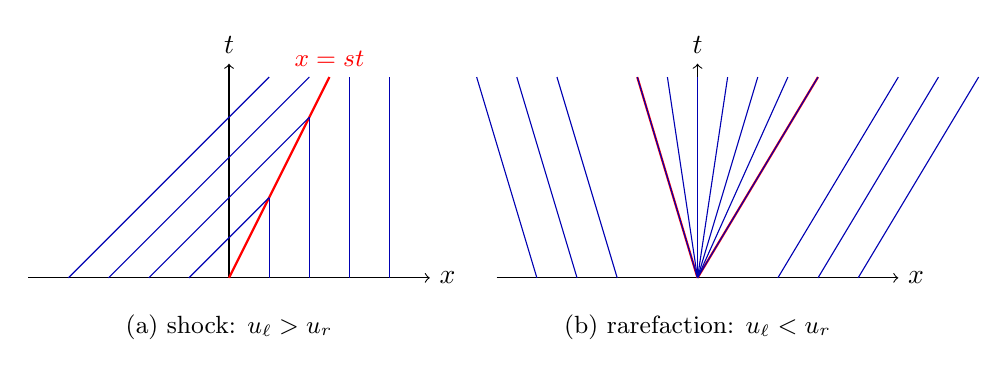
\begin{tikzpicture}[scale=0.85]
  % --- Shock case (left): u_l = 1, u_r = 0, s = 1/2 ---
  \begin{scope}
    \draw[->] (-3,0) -- (3,0) node[right] {$x$};
    \draw[->] (0,0) -- (0,3.2) node[above] {$t$};
    \draw[thick, red] (0,0) -- (1.5,3) node[above] {\small $x=st$};
    % left characteristics: speed u_l = 1, stop on hitting the shock x = t/2
    \foreach \xz in {-2.4,-1.8,-1.2,-0.6}{
      \pgfmathsetmacro{\tm}{min(3,-2*\xz)}
      \draw[blue!70!black] (\xz,0) -- ({\xz+\tm},\tm);
    }
    % right characteristics: speed u_r = 0 (vertical), stop on the shock
    \foreach \xz in {0.6,1.2,1.8,2.4}{
      \pgfmathsetmacro{\tm}{min(3,2*\xz)}
      \draw[blue!70!black] (\xz,0) -- (\xz,\tm);
    }
    \node[below] at (0,-0.4) {\small (a) shock: $u_\ell>u_r$};
  \end{scope}
  % --- Rarefaction case (right) ---
  \begin{scope}[xshift=7cm]
    \draw[->] (-3,0) -- (3,0) node[right] {$x$};
    \draw[->] (0,0) -- (0,3.2) node[above] {$t$};
    \draw[thick, red] (0,0) -- (-0.9,3);
    \draw[thick, red] (0,0) -- (1.8,3);
    \foreach \xz in {-2.4,-1.8,-1.2}{
      \draw[blue!70!black] (\xz,0) -- ({\xz-0.3*3},3);
    }
    \foreach \m in {0,1,...,6}{
      \draw[blue!70!black] (0,0) -- ({-0.9+\m*0.45},3);
    }
    \foreach \xz in {1.2,1.8,2.4}{
      \draw[blue!70!black] (\xz,0) -- ({\xz+0.6*3},3);
    }
    \node[below] at (0,-0.4) {\small (b) rarefaction: $u_\ell<u_r$};
  \end{scope}
\end{tikzpicture}
\caption{Characteristics for the two cases of
Theorem~\ref{thm:riemann-solution}. (a) $u_\ell=1$, $u_r=0$, $s=1/2$:
characteristics on both sides run into the shock $x=st$. (b) Characteristics
fan out from the origin.}
\label{fig:riemann-characteristics}
\end{figure}